\section{Predictive utility of the soft-state hierarchy}
\label{sec:softstate-study}

The experiment separates membership, local position, and
reconstruction enrichment. Every readout predicts the same future
observation using only its declared representation. This tests which
geometric observables a finite decoder can use without a retained
raw-history forecast supplying information outside those observables.
The comparison concerns fitted predictive accessibility; it does not
establish unrestricted information or Markov sufficiency.

\subsection{Representations and shared transformations}

Write $b_G=\Phi_G$ for the concatenated gates and $b_P$ for the
gate-weighted principal coordinates. Along with $d_K$ and $d_R$, these
give four raw blocks. Each block is centered and scaled on A alone,
with scale floor $10^{-6}$, and separately transformed by the radial
map in Equation~\eqref{eq:mechanism-main-radial}. Denote the resulting
blocks by $z_G,z_P,z_K,z_R$. An empty position block remains empty.
The four readout inputs are
\begin{equation}
 \chi_G=z_G,\qquad
 \chi_P=\operatorname{concat}(z_G,z_P),\qquad
 \chi_K^{\mathrm{sep}}=\operatorname{concat}(z_G,z_P,z_K),\qquad
 \chi_R^{\mathrm{sep}}=\operatorname{concat}(z_G,z_P,z_R).
 \label{eq:softstate-four-arms}
\end{equation}
We refer to these procedures as G, P, K, and R. The superscript
$\mathrm{sep}$ distinguishes the separately transformed gate and
position blocks from the earlier joint-common transformation in
Appendix~\ref{app:earlier-decoders}. The raw observables are unchanged.
The gate block is identical in all four inputs, and the position block
is identical in P, K, and R. Appending an observable block therefore
does not change the existing coordinates. K and R have the same nominal
width and readout architecture; this matching does not equate effective
function spaces, conditioning, or computational cost.

For each cap and horizon, an affine ridge head is fitted directly to the
observed A targets, with an unpenalized intercept. B selects a penalty
from $\{10^{-4},10^{-3},10^{-2},10^{-1},1\}$ independently for each arm
and horizon. There is no residual target, retained baseline, correction
multiplier, or calibration. C predictions are recorded as diagnostics
after all choices are fixed and do not affect fitting or selection.

\subsection{Validation-selected geometry and fresh evaluation}

Each candidate bank is fitted from A using the native construction in
Section~\ref{sec:reconstruction-method}. All four arms share its
reference histories, partitions, gates, projected kernels, and local
ranks. Candidate caps are $1,2,4,8,12$ at history width twelve; cap twenty
is an alias of twelve and does not receive an additional search slot.
The native variance and range reductions remain in force. Input
histories use A-fitted standardization, with no additional scaler search.

In the primary context, P selects one cap by mean B loss across horizons,
using the corresponding A-target population variance for normalization
and its previously selected horizon penalties. Exact ties choose the
first cap in ascending order. G, K, and R then use that same bank with
their own B-selected penalties. This estimates enrichment of a
validation-selected common representation. A secondary context allows
each arm to select its own cap from the same candidate fits; it measures
a complete procedure and cannot replace a primary comparison.

The fixed design specifies \SARepetitions\ independent repetitions of
four inherited laws and two added-noise levels, giving \SATasks\ task
suites. Histories have width twelve and horizons are $1,4,12$.
Independent A/B/C/D sets contain $64/32/32/128$ episodes of length
seventy-two. A/B/C retain at most $512/256/256$ rows; D retains all
$1,664$ origins. The observation laws, noise conventions, window
indexing, and paired-noise construction are those specified in
Appendix~\ref{app:reconstruction-results}. These fresh repetitions
extend evidence under known laws; they do not introduce new domains.
Earlier outcomes informed the design; the protocol excludes pooling earlier
observations into its inferential units.

Source, configuration, analysis, and the repetition budget were frozen
and the scientific source was published before production data generation.
The complete A/B fitted-state roster was sealed before D generation,
and all D forecasts were sealed before terminal scoring.
Source hashes and phase records document this ordering;
they do not constitute independent oversight or cryptographic target
isolation. The pipeline retains candidate choices, portable fitted states,
forecasts, numerical recoveries, and complete fitting-and-selection costs.

\subsection{Primary comparison family}

Task losses average variance-normalized squared error over origins and
horizons. Within each repetition, nonlinear losses average the three
nonlinear laws and both noise levels equally; the linear control averages
its two noise levels. The independent units are the
\SARepetitions\ repetition aggregates, not overlapping windows.
There is one family of four primary claims: nonlinear P versus G, K
versus P, and K versus R at a $3\%$ superiority margin, and linear K
versus P at a $5\%$ noninferiority margin. These are inherited research
thresholds rather than deployment-derived costs.

For each claim, let $d_r=L_{a,r}-cL_{b,r}$, where $a$ and $b$ are the
candidate and reference and $c=0.97$ for superiority or $1.05$ for
noninferiority. With $n=\SARepetitions$, the one-sided upper endpoint is
\begin{equation}
 U=\bar d+t_{n-1,1-0.05/4}\,s_d/\sqrt n.
 \label{eq:softstate-primary-bound}
\end{equation}
Here $t_{\nu,p}$ is the $p$ quantile of a Student distribution with
$\nu$ degrees of freedom. A criterion is established only if $U<0$.
This Bonferroni family uses
the paired-$t$ model for independent repetition aggregates; its finite
sample accuracy depends on that approximation. Percentage gains are
$100\{1-\overline L_a/\overline L_b\}$. Independent-cap, law, noise,
horizon, and resource analyses are secondary and descriptive. An
unestablished margin is not evidence of equivalence.

\subsection{Results and their scope}

Table~\ref{tab:softstate-primary} reports all four primary comparisons.
P reduces nonlinear loss relative to G by \SAGainPG\%, and K reduces
loss relative to P by \SAGainKP\%. Both simultaneous upper endpoints
are below zero, establishing the respective $3\%$ margins.
The mean K/R difference is much smaller: K improves R by only
\SAGainKR\%, with a positive margin-adjusted upper endpoint. The
KAHM-specific $3\%$ superiority criterion is not established.
On the linear control, K's loss exceeds P's by $1.11\%$, while the
upper endpoint for the $5\%$ noninferiority criterion remains negative.
The complete family therefore establishes \SACriteriaEstablished\ of
\SAFamilySize\ criteria, supporting position and KAHM enrichment
relative to their nested inputs under this procedure, without
establishing superiority over matched RBF enrichment.

\begin{table}[t]
\centering\small
\caption{Complete primary family for the P-selected shared bank.
Gain is $100(1-\overline L_a/\overline L_b)$; negative gain denotes
higher candidate loss. The margin-adjusted difference is
$d=L_a-cL_b$, with $c=0.97$ for superiority and $1.05$ for
noninferiority. A criterion is established only when its simultaneous
one-sided upper endpoint is below zero. The independent units are
the \SARepetitions\ repetition aggregates.}
\label{tab:softstate-primary}
% Generated by build_soft_state_assets.py; do not edit.
% Shared caps; d=L_candidate-factor*L_reference. Four Bonferroni one-sided paired-t upper bounds; met iff upper<0.
\begin{tabular}{@{}lllrrrc@{}}
\toprule
Population & Contrast & Criterion & Gain (\%) & $\bar d$ & Upper bound & Met \\
\midrule
Nonlinear & P vs G & 3\% sup. & 69.20 & \ensuremath{-0.06545} & \ensuremath{-0.06253} & Yes \\
Nonlinear & K vs P & 3\% sup. & 10.46 & \ensuremath{-0.002271} & \ensuremath{-0.001987} & Yes \\
Nonlinear & K vs R & 3\% sup. & 0.03 & 0.0008103 & 0.000981 & No \\
Linear & K vs P & 5\% NI & \ensuremath{-1.11} & \ensuremath{-0.03542} & \ensuremath{-0.03134} & Yes \\
\bottomrule
\end{tabular}

\end{table}

\begin{table}[t]
\centering\small
\caption{Mean variance-normalized terminal loss and standard deviation
across repetitions. The shared bank is selected by P. Independent
per-arm cap selection is a secondary procedure comparison; its
outcomes cannot replace a primary criterion. Standard deviations
describe repetitions and are not confidence intervals.}
\label{tab:softstate-aggregate}
% Generated by build_soft_state_assets.py; do not edit.
% D SMSE; SD across 32 complete repetitions, not a confidence interval. Independent caps are secondary.
\begin{tabular}{@{}llrrrr@{}}
\toprule
Cap rule & Arm & Nonlinear mean & SD & Linear mean & SD \\
\midrule
Shared & G & 0.0988703 & 0.00788637 & 0.939042 & 0.0484704 \\
Shared & P & 0.0304507 & 0.00150099 & 0.910921 & 0.0513907 \\
Shared & K & 0.027266 & 0.00123317 & 0.921045 & 0.0526607 \\
Shared & R & 0.027274 & 0.00127755 & 0.915866 & 0.0512334 \\
\addlinespace
Independent & G & 0.0988703 & 0.00788637 & 0.939042 & 0.0484704 \\
Independent & P & 0.0304507 & 0.00150099 & 0.910921 & 0.0513907 \\
Independent & K & 0.0267546 & 0.00120524 & 0.914936 & 0.0511589 \\
Independent & R & 0.0267507 & 0.00129299 & 0.91589 & 0.0521994 \\
\bottomrule
\end{tabular}

\end{table}

Table~\ref{tab:softstate-aggregate} shows that independent cap selection
reduces nonlinear K and R losses to \SALossIndependentNonlinearK\ and
\SALossIndependentNonlinearR\ respectively. K's descriptive gain over
P becomes $12.14\%$, while its K/R gain becomes $-0.01\%$.
These point estimates do not establish equivalence or a primary
advantage under a different selection rule. G's forecasts are identical
across caps in this construction: the shared seed and references leave
the center-distance gates unchanged. Its independent choice of cap one
is consequently a tie-breaking outcome, not evidence that rank one
best captures the dynamics. P's independently chosen cap is the
primary cap by definition.

The aggregate gains are heterogeneous
(Figure~\ref{fig:softstate-conditions}). K improves P on both oscillator
laws at both noise levels, but worsens P on nonlinear autoregression
at both levels. It improves matched R in three of the six nonlinear
law/noise cells and worsens it in the other three. By horizon, nonlinear
K/P loss is higher at $h=1$, nearly unchanged at $h=4$, and lower at
$h=12$. These are descriptive decompositions of the complete results,
not additional confirmed subpopulation claims. They show why a
positive aggregate enrichment result does not justify universal
deployment of the departure block.

\begin{figure}[t]
\centering
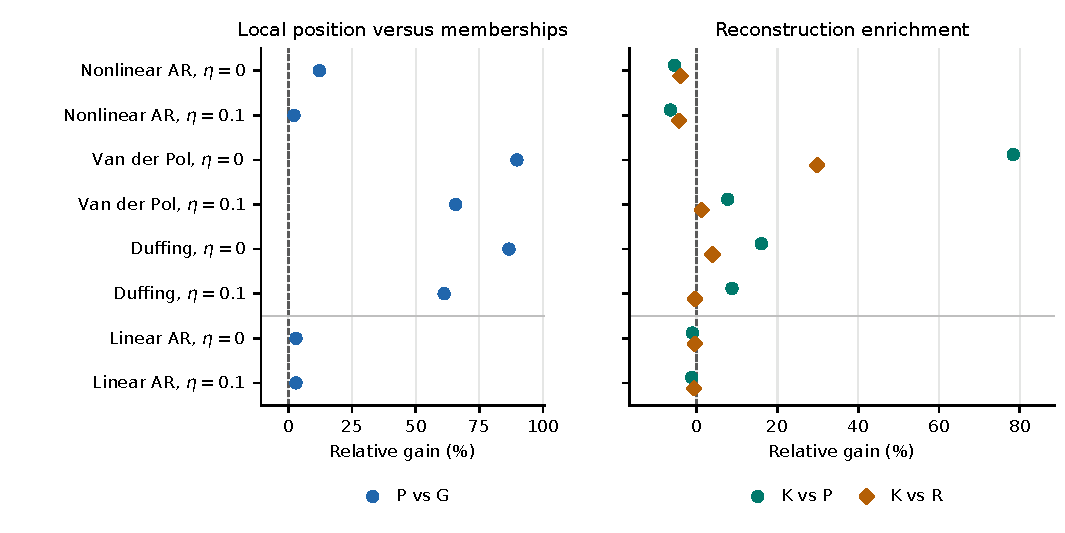
\includegraphics[width=\linewidth]{generated/soft_state_ablation/condition_gains.pdf}
\caption{Descriptive shared-bank gains by observation law and added
noise. Positive values favor the candidate. Each point uses all
\SARepetitions\ repetitions and averages the three horizons; the
condition displays have no separate confirmatory status. The complete
primary confidence family is in Table~\ref{tab:softstate-primary}.}
\label{fig:softstate-conditions}
\end{figure}

The Supplementary Studies reports all law/noise and horizon losses,
both cap-selection contexts, dimensions, and resource accounting.
Selected G, P, and K/R widths are $14$, $28$--$182$, and
$196$--$350$, respectively, for history width twelve. These descriptors
are therefore not a compression claim. Complete fitting and selection
uses \SAFitWallHours\ summed worker wall hours and
\SAFitCPUHours\ CPU hours; D prediction adds
\SAPredictionWallSeconds\ summed worker wall seconds.
Peak measured worker memory is \SAPeakWorkerRSSMiB\ MiB. These costs
include all candidates and reused geometry. Summed worker time is
not elapsed parallel runtime, and the measurements do not identify
isolated K versus R deployment costs. Preparation, audit and document
production are outside these fitting-and-prediction measurements.

Every planned task and primary contrast is retained. The source,
budget, menu and comparison family were unchanged after publication;
unfavorable comparisons did not trigger additional repetitions.
The experiment establishes finite direct-readout utility under the
specified laws and allocation. It does not test autonomous coordinate
propagation, Markov sufficiency, or a generally preferable forecasting
policy.
